\section{Experiment}

\subsection{Enverionment}
\begin{frame}
	\frametitle{Enverionment}
	\begin{itemize}
		\item Intel Xeon E5-2670 2.6GHz, 64GB Memory
		\item Intel C++ Compiler
		\item The environment variable \texttt{KMP\_AFFINITY} was used 
			to control thread locality when needed.
	\end{itemize}
\end{frame}

\begin{frame}
	\frametitle{Large Graphs}
	\begin{figure}
		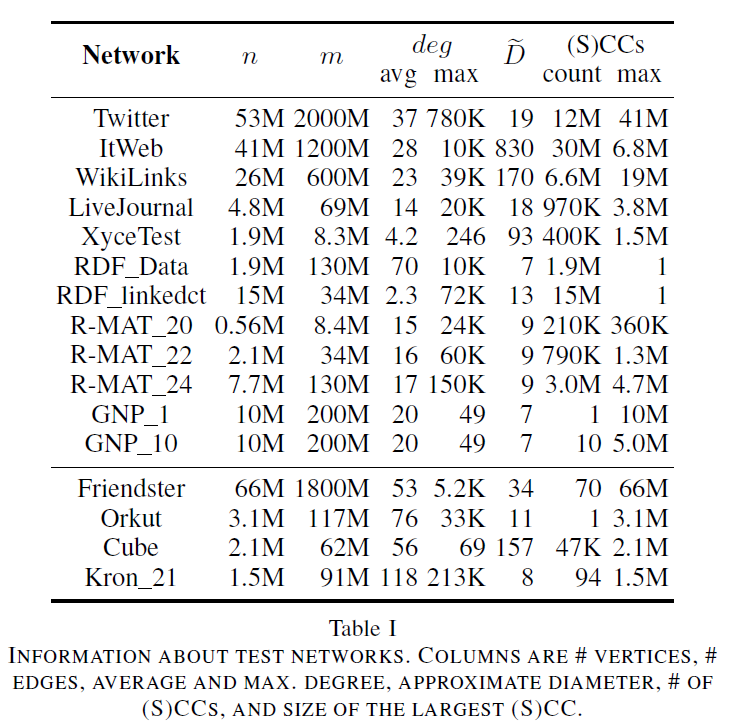
\includegraphics[scale=0.35]{figure/fig-test-graph.png}
	\end{figure}
\end{frame}

\subsection{Result}
\begin{frame}
	\frametitle{Result}
	\begin{figure}
		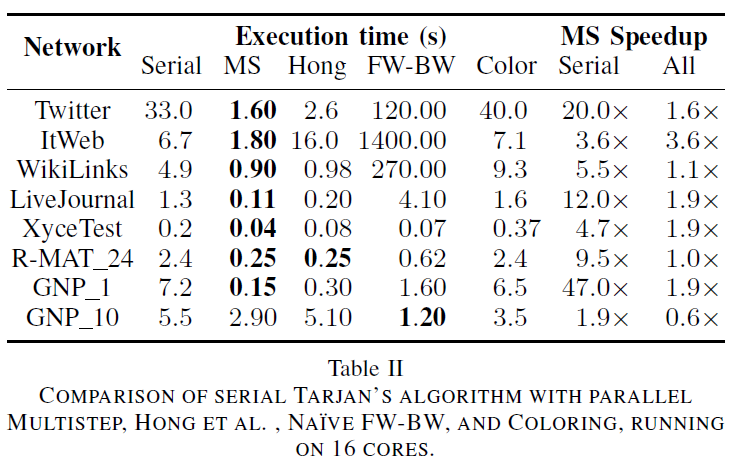
\includegraphics[scale=0.35]{figure/fig-result.png}
	\end{figure}
\end{frame}

\begin{frame}
	\frametitle{Time Proportion in Multistep Algorithm}
	\begin{figure}
		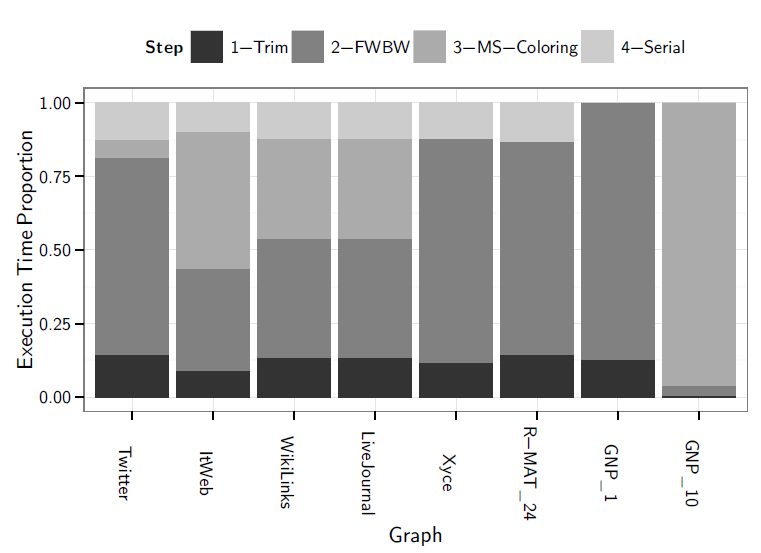
\includegraphics[scale=0.40]{figure/fig-result-p1.png}
	\end{figure}
\end{frame}

\begin{frame}
	\frametitle{Trimming Procedures in Multistep Algorithm}
	\begin{figure}
		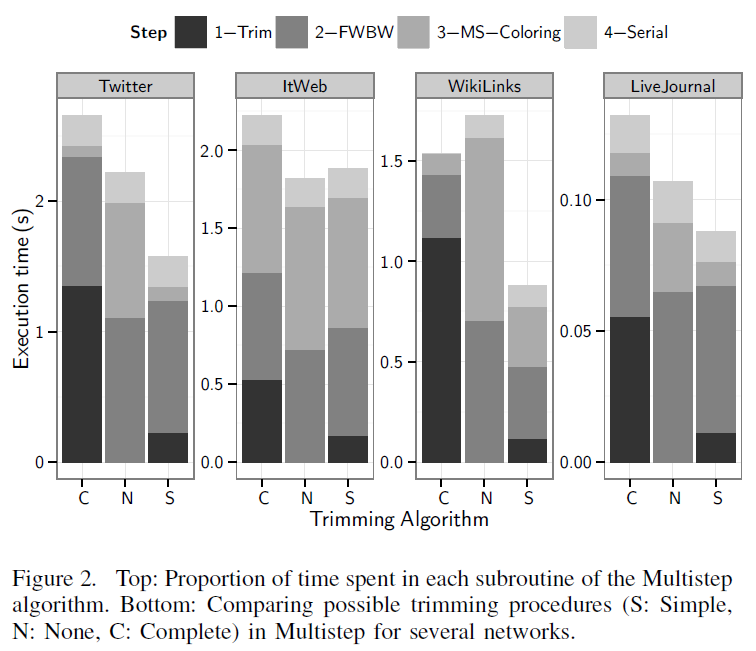
\includegraphics[scale=0.40]{figure/fig-result-p2.png}
	\end{figure}
\end{frame}

\begin{frame}
	\frametitle{Strongly Connected Component}
	\begin{figure}
		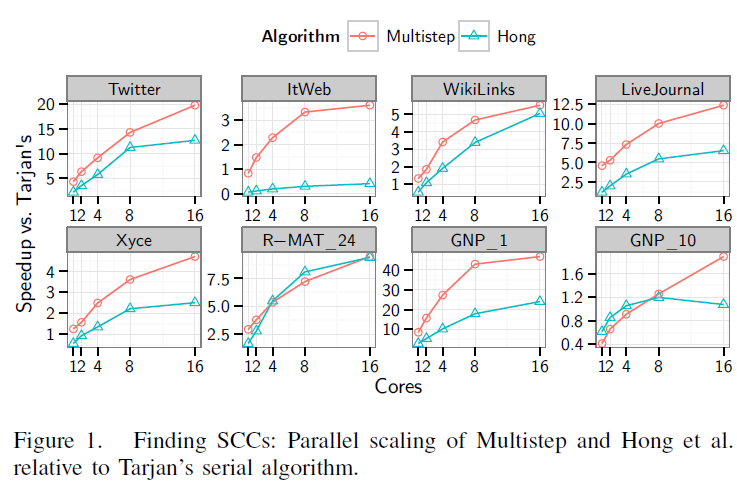
\includegraphics[scale=0.40]{figure/fig-result-f1.png}
	\end{figure}
\end{frame}

\begin{frame}
	\frametitle{Connected Component}
	\begin{figure}
		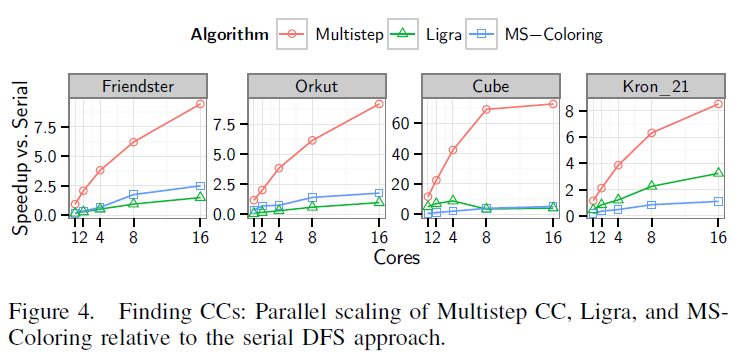
\includegraphics[scale=0.40]{figure/fig-result-f2.png}
	\end{figure}
\end{frame}

\begin{frame}
	\frametitle{Weakly Connected Component}
	\begin{figure}
		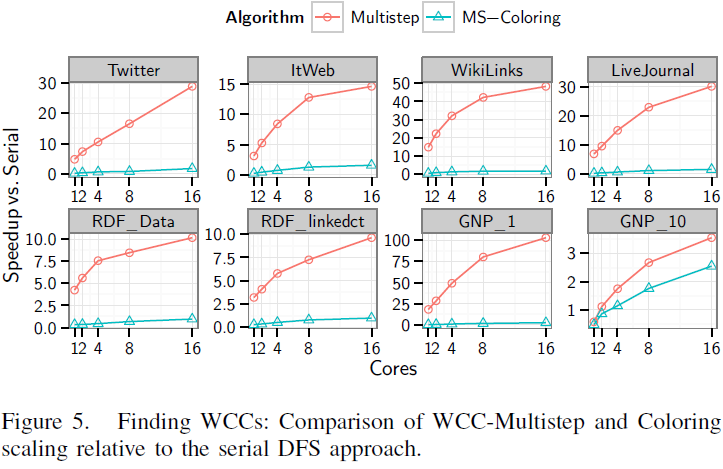
\includegraphics[scale=0.40]{figure/fig-result-f3.png}
	\end{figure}
\end{frame}

\begin{frame}
	\frametitle{Biconnected Connected Component}
	\begin{figure}
		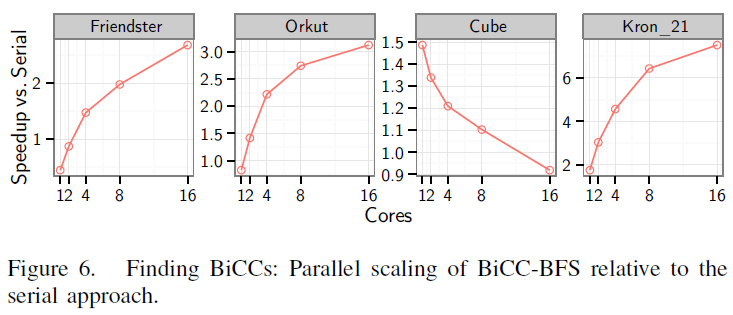
\includegraphics[scale=0.40]{figure/fig-result-f4.png}
	\end{figure}
\end{frame}